\documentclass[11pt,a4paper]{article}

\usepackage[margin=2.3cm]{geometry}
\usepackage[T1]{fontenc}
\usepackage[utf8]{inputenc}
\usepackage{lmodern}
\usepackage{textcomp}
\usepackage{microtype}
\usepackage{amsmath}
\usepackage{booktabs}
\usepackage{graphicx}
\usepackage{hyperref}
\usepackage{xcolor}
\usepackage{listings}

\hypersetup{
    colorlinks=true,
    linkcolor=black!70,
    urlcolor=blue!60!black,
}

\lstset{
    basicstyle=\ttfamily\footnotesize,
    columns=fullflexible,
    keepspaces=true,
    breaklines=true,
    showstringspaces=false,
    frame=single,
    framesep=3pt,
    xleftmargin=6pt,
}

\title{\vspace{-1cm}Assignment 3: Serverless Customer Review Processing\\
       \large Event-Driven Profanity Check and Sentiment Analysis on MiniStack}
\author{
Group 48, Data-Intensive Computing, TU Wien, SS~2026\\[2pt]
\small
Aaradhaya Arora (12534787) \quad
Ekaterina Dobrynina (12332276) \quad
Gopinath Hariharasudhan (52202173) \\[1pt]
\small
Serhii Slutu (12537831) \quad
Sofia Zubkova (12534780)
}
\date{\today}

\begin{document}
\maketitle

\vspace{-0.4cm}

\noindent\textbf{AI disclosure.}
We used various AI tools (e.g., ChatGPT, Claude via Cursor) as a support tool while working on this
assignment. Its use was limited to text polishing (grammar, wording), to
debugging help when we were stuck, and to drafting assistance for this
report. The serverless architecture, the choice of AWS services and
triggers, the Lambda implementations, and all design decisions were made
by us; the models did not generate the solution on their own, they were
used purely as assistance.

\vspace{0.2cm}

%==============================================================
\section{Introduction}
%==============================================================

This assignment asks us to build an event-driven serverless application
that ingests customer product reviews and performs three main tasks on
each review: text preprocessing, profanity checking, and sentiment
analysis. In addition, the system must track how many impolite reviews
each customer submits and ban users who exceed a configurable threshold.

We implement the application on \emph{MiniStack}, a local AWS emulator
running on the LBD cluster. The design follows the course tutorial:
Lambda functions are deployed independently, communicate only through
AWS platform events (S3 object creation and DynamoDB updates), and read
all resource names from the Systems Manager (SSM) Parameter Store rather
than hard-coding them.

The development set \texttt{reviews\_devset.json} contains 78\,829
Amazon-style review records. Each review is uploaded individually to S3,
which starts the processing chain. In the rest of this report we describe
the problem, our architecture and implementation, and the numbers
produced on the development set.

%==============================================================
\section{Problem Overview}
%==============================================================

\paragraph{Input.}  Each review is a JSON object. The fields relevant to
this assignment are \texttt{reviewText} (the main review body),
\texttt{summary} (a short headline), \texttt{overall} (a numeric star
rating), and \texttt{reviewerID} (the customer identifier).

\paragraph{Preprocessing.}  The first Lambda tokenizes the combined text
of \texttt{summary} and \texttt{reviewText}, removes English stop words,
POS-tags the remaining tokens, and lemmatizes them with WordNet. The
enriched record is written to a processed-reviews S3 bucket.

\paragraph{Profanity check.}  The second Lambda scans the same text
fields for bad words using the \texttt{profanityfilter} library, marks
each review as \texttt{clean} or \texttt{impolite}, stores the result
in a DynamoDB reviews table, and increments an impolite-review counter
for the submitting user. When a user's count exceeds the ban threshold
(3 impolite reviews, i.e.\ more than three), the user is marked as
banned in a separate users table.

\paragraph{Sentiment analysis.}  The third Lambda runs NLTK's VADER
sentiment analyser on the text fields, classifies each review as
\texttt{positive}, \texttt{neutral}, or \texttt{negative}, and compares
the text sentiment against the numeric \texttt{overall} rating to record
whether they agree.

\paragraph{Constraints.}  The assignment requires at least three Lambda
functions, an event-driven chain starting from a single S3 upload, SSM
for configuration, and automated integration tests. The reported results
must be computed from \texttt{reviews\_devset.json} only.

%==============================================================
\section{Methodology and Approach}
%==============================================================

\subsection{Architecture}

Figure~\ref{fig:architecture} shows the complete function chain and how
each component interacts with the AWS platform services. No Lambda
invokes another directly; every hand-off is mediated by an S3 or
DynamoDB event.

\begin{figure}[h]
    \centering
    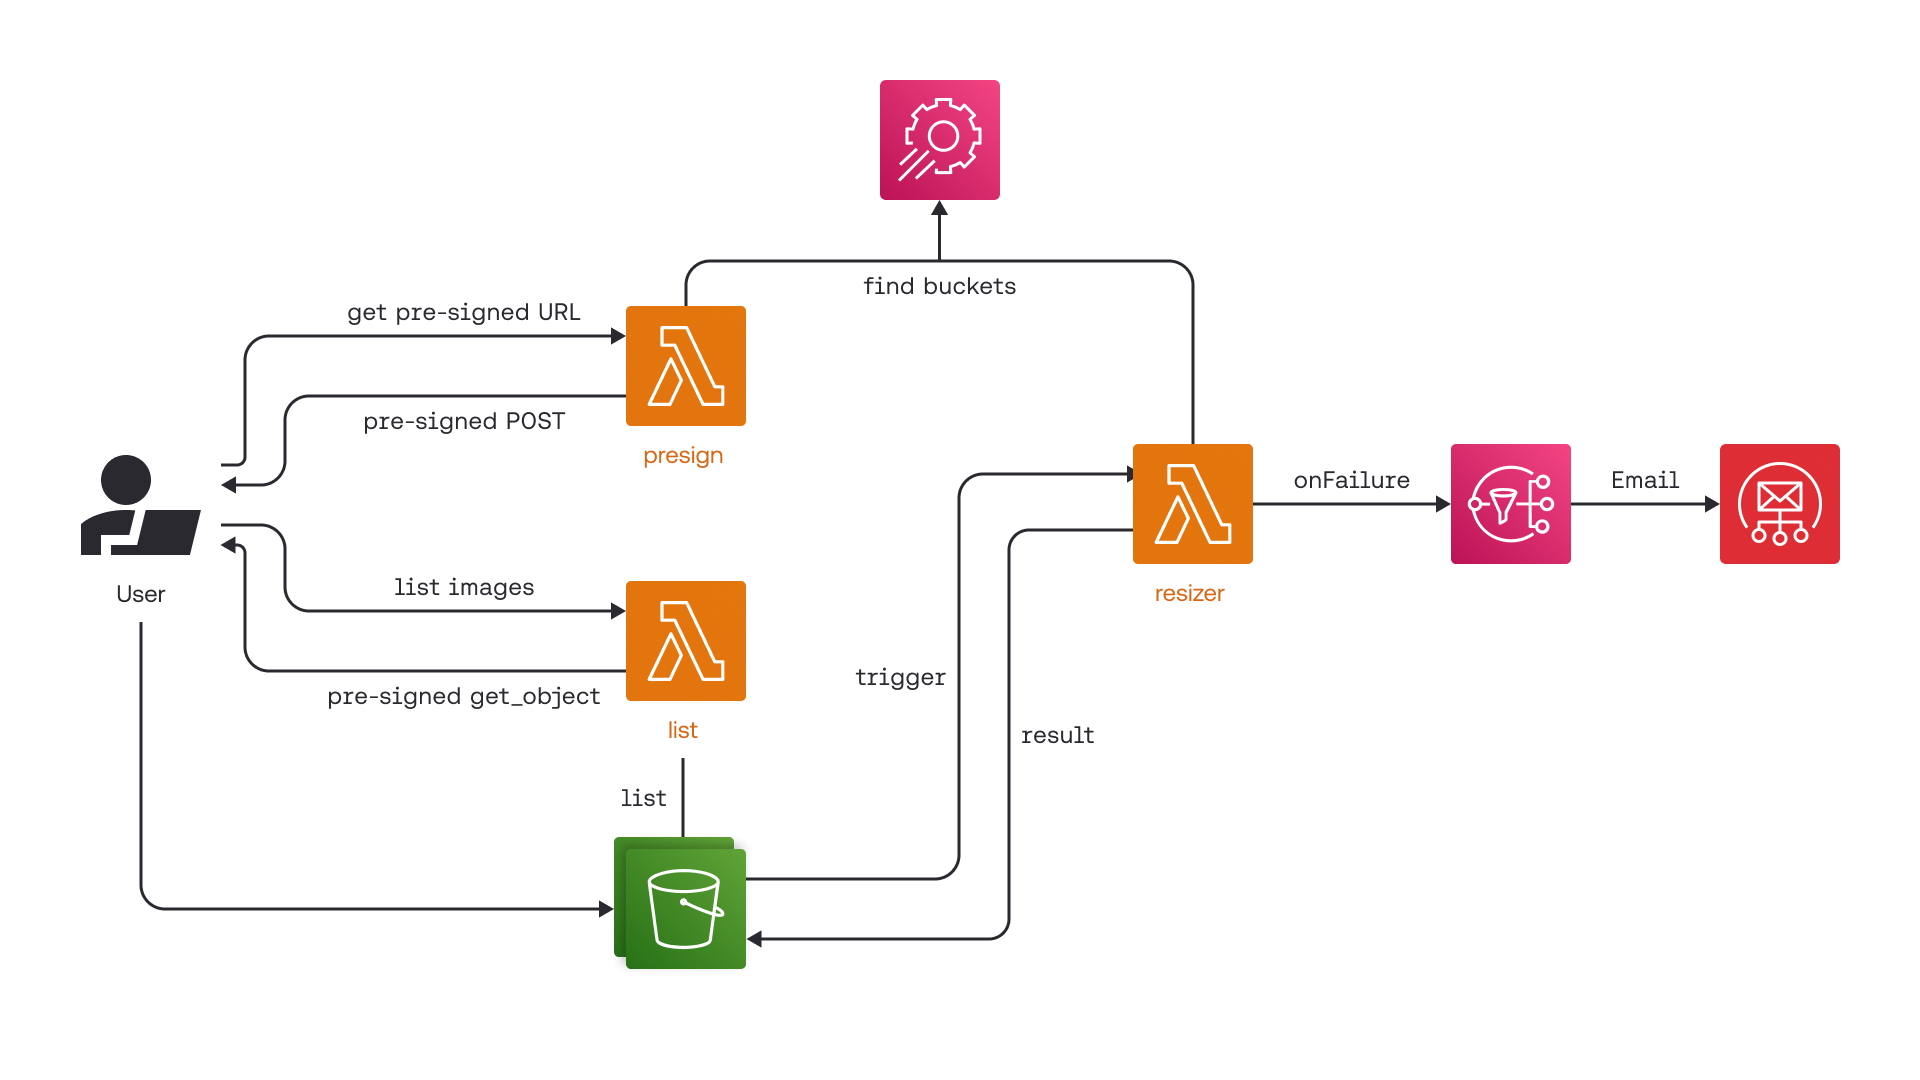
\includegraphics[width=\textwidth]{architecture.png}
    \caption{Serverless review-processing architecture. Uploading one
             review JSON to the raw bucket triggers preprocessing; the
             resulting object in the processed bucket triggers
             profanity-check and sentiment-analysis in parallel. Both
             downstream Lambdas write to DynamoDB. Bucket and table names
             are resolved at runtime from SSM Parameter Store.}
    \label{fig:architecture}
\end{figure}

\subsection{Trigger chain}

\begin{enumerate}
    \item \textbf{Upload.} A driver script (or an integration test) puts
          one review JSON into the \emph{raw reviews} S3 bucket.
    \item \textbf{Preprocessing} (\texttt{preprocessing} Lambda) is
          triggered by \texttt{s3:ObjectCreated}. It reads the object,
          preprocesses the text, assigns a \texttt{reviewId} (using an
          optional \texttt{sourceId} tag for devset rows), and writes the
          enriched JSON to the \emph{processed reviews} bucket.
    \item \textbf{Profanity check} (\texttt{profanity-check} Lambda) and
          \textbf{sentiment analysis} (\texttt{sentiment-analysis}
          Lambda) both listen on the processed bucket's
          \texttt{ObjectCreated} event and run \emph{in parallel} on the
          same object.
    \item \textbf{DynamoDB writes.} Profanity-check creates or updates a
          row in the reviews table (setting \texttt{profanityCheck} and
          user metadata) and updates the user's impolite count in the
          users table. Sentiment-analysis updates the same reviews row
          with \texttt{sentiment}, \texttt{sentimentScore}, and
          \texttt{ratingSentimentAgreement}.
\end{enumerate}

Because the two downstream Lambdas can finish in either order, both use
DynamoDB \texttt{update\_item} with \texttt{if\_not\_exists} guards so
that neither overwrites fields already written by the other.

\subsection{Configuration via SSM}

All infrastructure names are stored in SSM and read at Lambda cold
start:

\begin{lstlisting}[caption={SSM parameters used by the application}]
/dic-reviews-app/buckets/raw
/dic-reviews-app/buckets/processed
/dic-reviews-app/tables/reviews
/dic-reviews-app/tables/users
/dic-reviews-app/config/ban-threshold
\end{lstlisting}

The deployment script \texttt{run.sh} creates the buckets and tables,
writes these parameters, packages each Lambda (NLTK and
\texttt{profanityfilter} dependencies bundled as Linux wheels), and
registers the S3 notification configurations.

\subsection{Libraries and design choices}

\begin{itemize}
    \item \textbf{NLTK} for tokenization, POS tagging, lemmatization
          (preprocessing) and VADER sentiment scoring (sentiment
          analysis). NLTK data packages are downloaded to \texttt{/tmp}
          on first invocation inside the Lambda container.
    \item \textbf{profanityfilter} for the profanity check. The filter
          operates on the raw \texttt{summary} and \texttt{reviewText}
          strings (not on the lemmatized tokens), which keeps behaviour
          aligned with the assignment's intent.
    \item \textbf{Parallel S3 triggers} for profanity-check and
          sentiment-analysis. An earlier design used a DynamoDB Stream
          on the reviews table to trigger sentiment analysis, but under
          high load on MiniStack the stream backlog caused timeouts when
          processing the full devset. Triggering both functions from the
          processed bucket is still fully compliant with the assignment
          requirement that invocations be driven by S3 and/or DynamoDB
          events.
    \item \textbf{Deterministic devset IDs.} The upload script tags each
          devset review with \texttt{sourceId = devset-NNNNNN}, which
          preprocessing propagates as \texttt{reviewId}. This lets the
          tally script isolate devset-derived rows from ad-hoc test
          uploads without extra bookkeeping.
\end{itemize}

\subsection{Testing}

Integration tests in \texttt{tests/test\_integration.py} upload synthetic
reviews to the raw bucket and poll DynamoDB until the expected state
appears. They cover:

\begin{itemize}
    \item a clean, positive review flowing through all three stages;
    \item a rating/sentiment disagreement (5-star rating with negative
          text);
    \item profanity detection (\texttt{damn} in the review text);
    \item automatic banning after four impolite reviews from the same
          user (threshold is \texttt{> 3}).
\end{itemize}

To produce the assignment results, \texttt{scripts/run\_devset.py}
uploads every review from \texttt{reviews\_devset.json} individually,
and \texttt{scripts/tally\_results.py --wait} polls until all devset
rows have a final sentiment label.

%==============================================================
\section{Results}
%==============================================================

We processed the full development set on MiniStack after deploying with
\texttt{run.sh}. Table~\ref{tab:results} summarises the numbers; they
match the output written to \texttt{data/results\_summary.json}.

\begin{table}[h]
    \centering
    \caption{Results on \texttt{reviews\_devset.json} (78\,829 reviews).}
    \label{tab:results}
    \begin{tabular}{@{}lr@{}}
        \toprule
        Metric & Count \\
        \midrule
        Total reviews processed        & 78\,829 \\
        Positive sentiment           & 67\,522 \\
        Neutral sentiment            &  1\,573 \\
        Negative sentiment           &  9\,734 \\
        Reviews failing profanity check &  3\,135 \\
        \bottomrule
    \end{tabular}
\end{table}

\paragraph{Banned users.}  One user from the development set exceeded the
ban threshold: \texttt{A320TMDV6KCFU} submitted four impolite reviews
(\texttt{impoliteCount = 4}) and was marked \texttt{banned = true} in
the users table.

\paragraph{Rating vs.\ text sentiment.}  For every devset review that
carried an \texttt{overall} rating, we also recorded whether the VADER
label agreed with the rating bucket (rating $\leq 2$ $\rightarrow$
negative, $\geq 4$ $\rightarrow$ positive, otherwise neutral). Across
78\,829 compared reviews, 15\,469 showed a disagreement between the
star rating and the text sentiment. This is a useful sanity check that the
\texttt{overall} field is being taken into account as required.

%==============================================================
\section{Conclusions}
%==============================================================

We built a three-Lambda serverless pipeline on MiniStack that
preprocesses, profanity-checks, and sentiment-analyses customer reviews
in a fully event-driven way. S3 uploads start the chain; parallel S3
triggers fan out profanity checking and sentiment analysis; DynamoDB
stores the final state and tracks user bans. All configuration is
externalised to SSM, and integration tests verify the main behaviours.

On the 78\,829-review development set the pipeline classified the
majority of reviews as positive (67\,522), flagged 3\,135 as impolite,
and banned one repeat offender. The implementation re-deploys cleanly
after every MiniStack restart via \texttt{run.sh}, which matches the
ephemeral nature of the emulator environment described in the assignment.

\end{document}
